\chapter{Results and Discussion}\label{chap:results}



\section{Underactuated PID Control}\label{sec:PID_results}

The underactuated PID controller is first implemented in simulation according \Cref{sec:sim_setup}. \Cref{fig:PID_sim_results} shows key system states during the balancing procedure. The platform's roll initially drops to $-17^{\circ}$ due to gravity, but the proportional action in the action in the controller quickly compensates as seen by the rapid spike in $\Delta\,d_y$. After about 45 seconds, the platform's roll, pitch, and horizontal body rates converge to 0. The sliding mass positions additionally settle to a constant value, indicating the gravitional torque has been driven towards 0. The simulation also verifies that the roll and pitch travel limits of the simulator ($\pm20^{\circ}$) have not been violated, and that the maximum speed and travel limits of the sliding masses have not been violated, even under a relatively large inital imbalance.

\begin{figure}[p!]
    \centering
    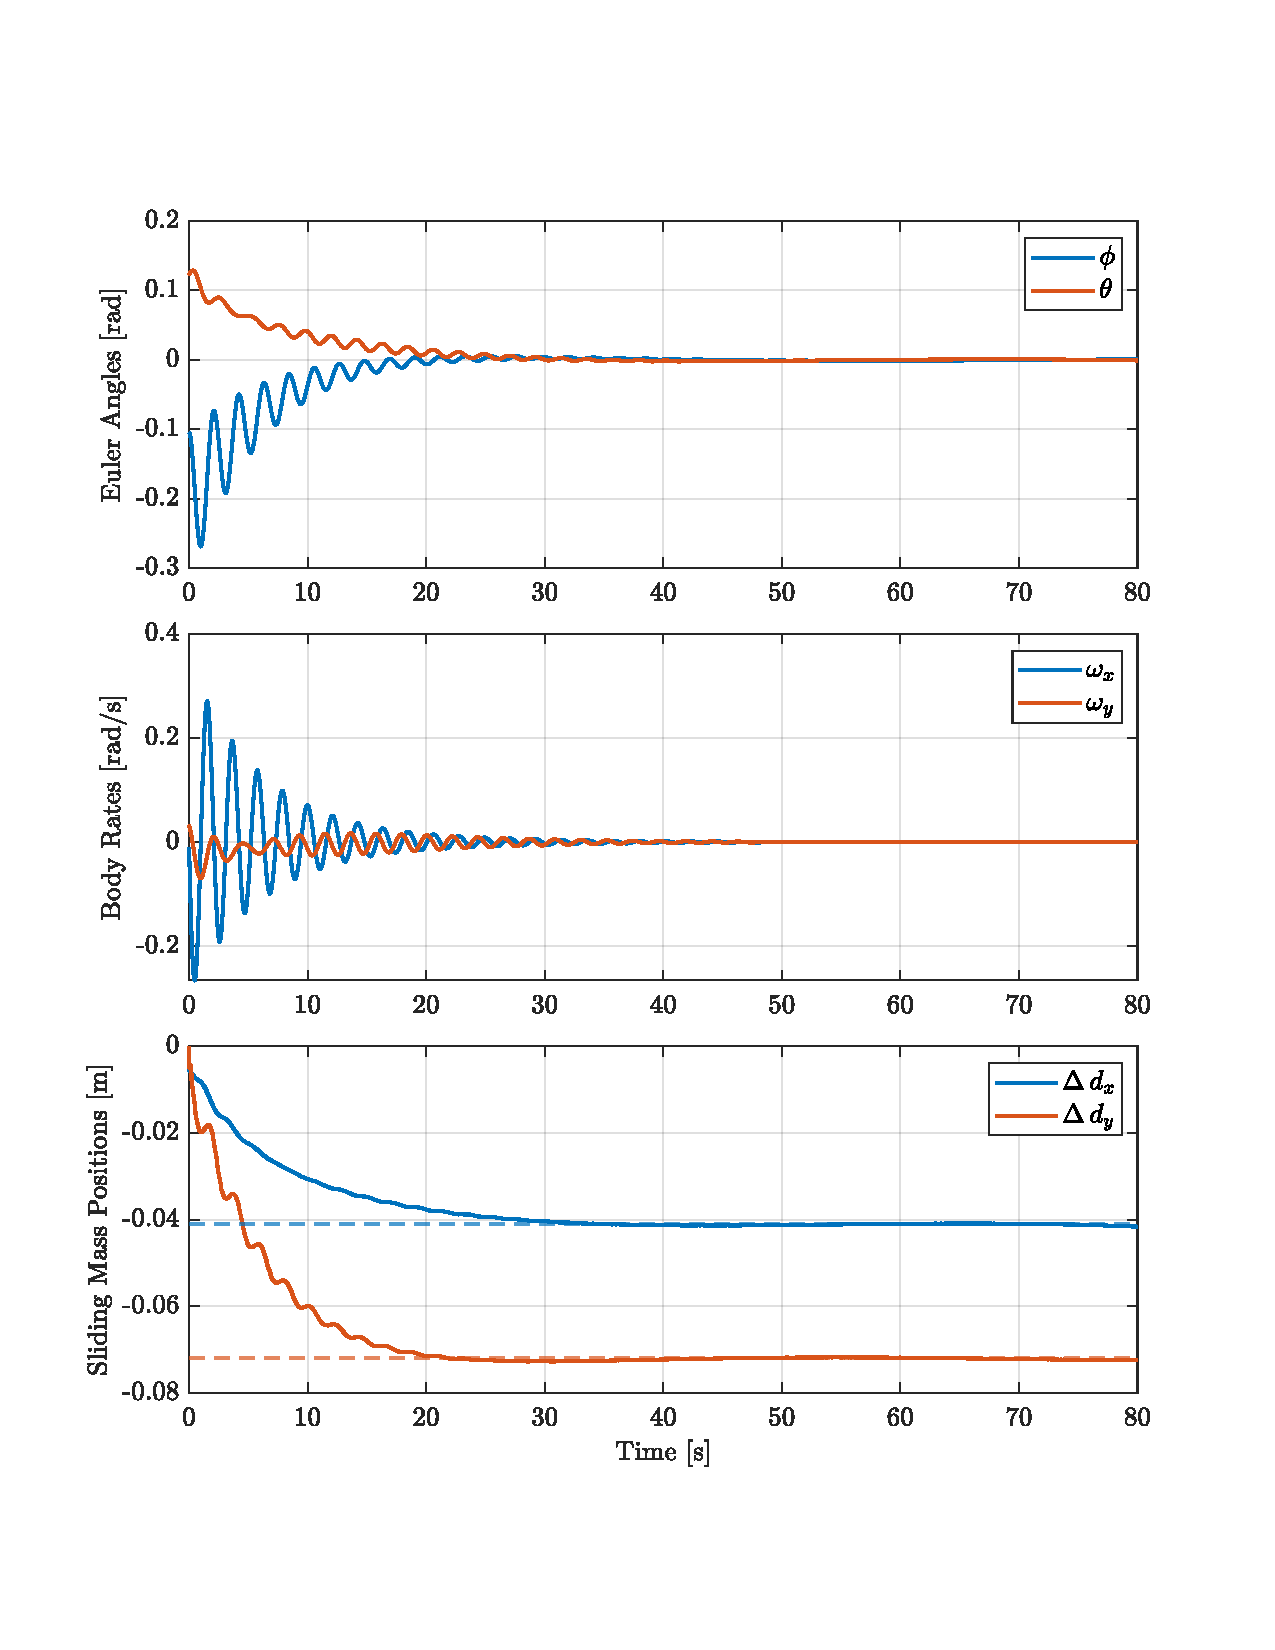
\includegraphics[width=\linewidth]{plots/PID_sim_results.pdf}
    \caption{Simulated balancing results using PID control}
    \label{fig:PID_sim_results}
\end{figure}

\begin{figure}[p!]
    \centering
    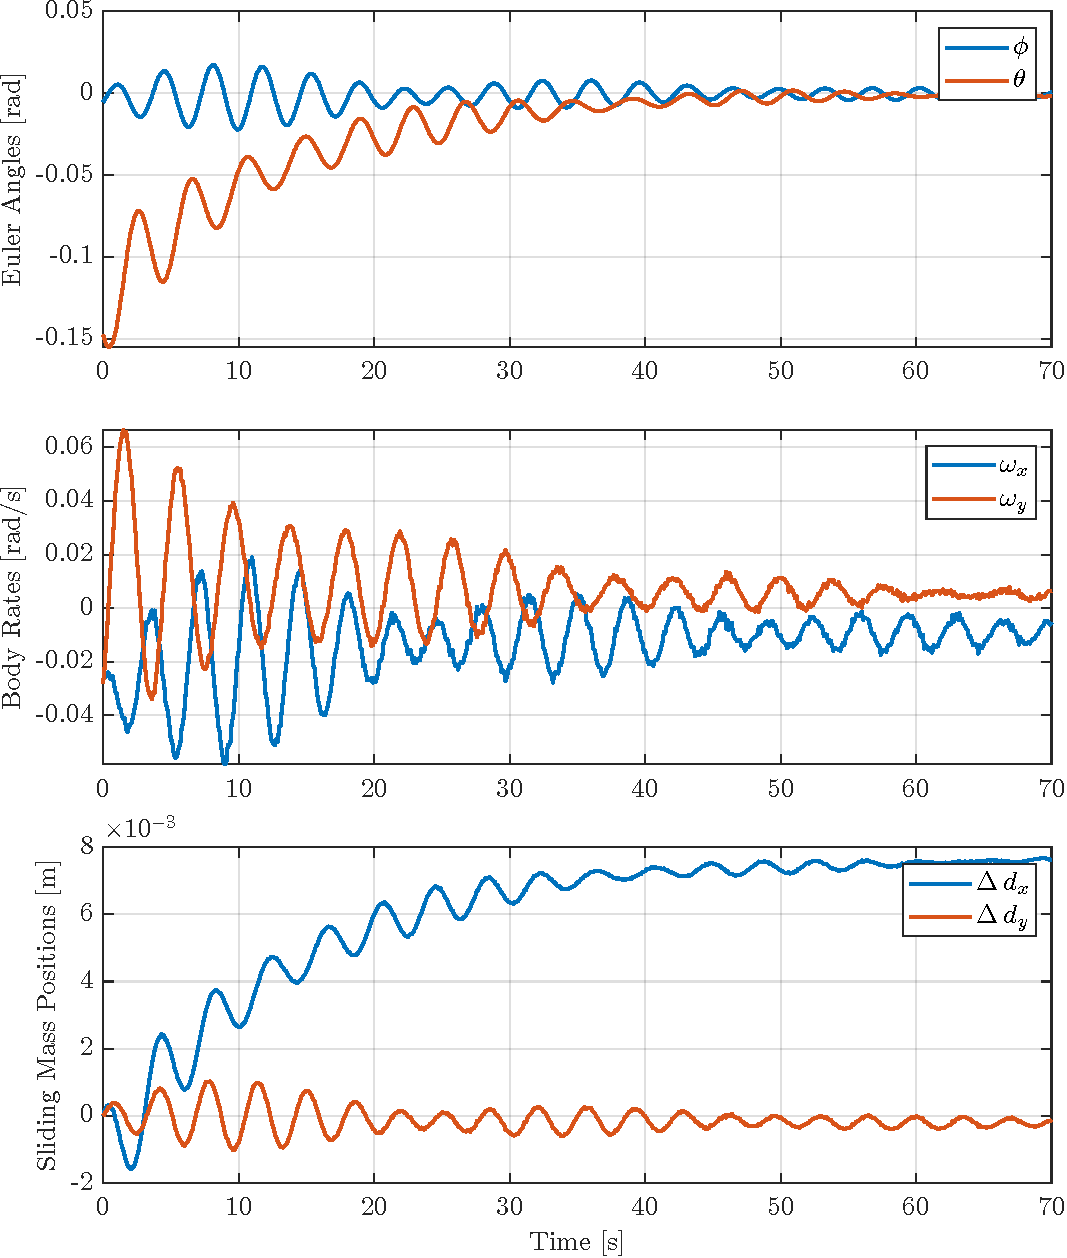
\includegraphics[width=\linewidth]{plots/PID_hardware_results.pdf}
    \caption{Experimental balancing results using PID control}
    \label{fig:PID_hardware_results}
\end{figure}

\begin{figure}[h]
    \centering
    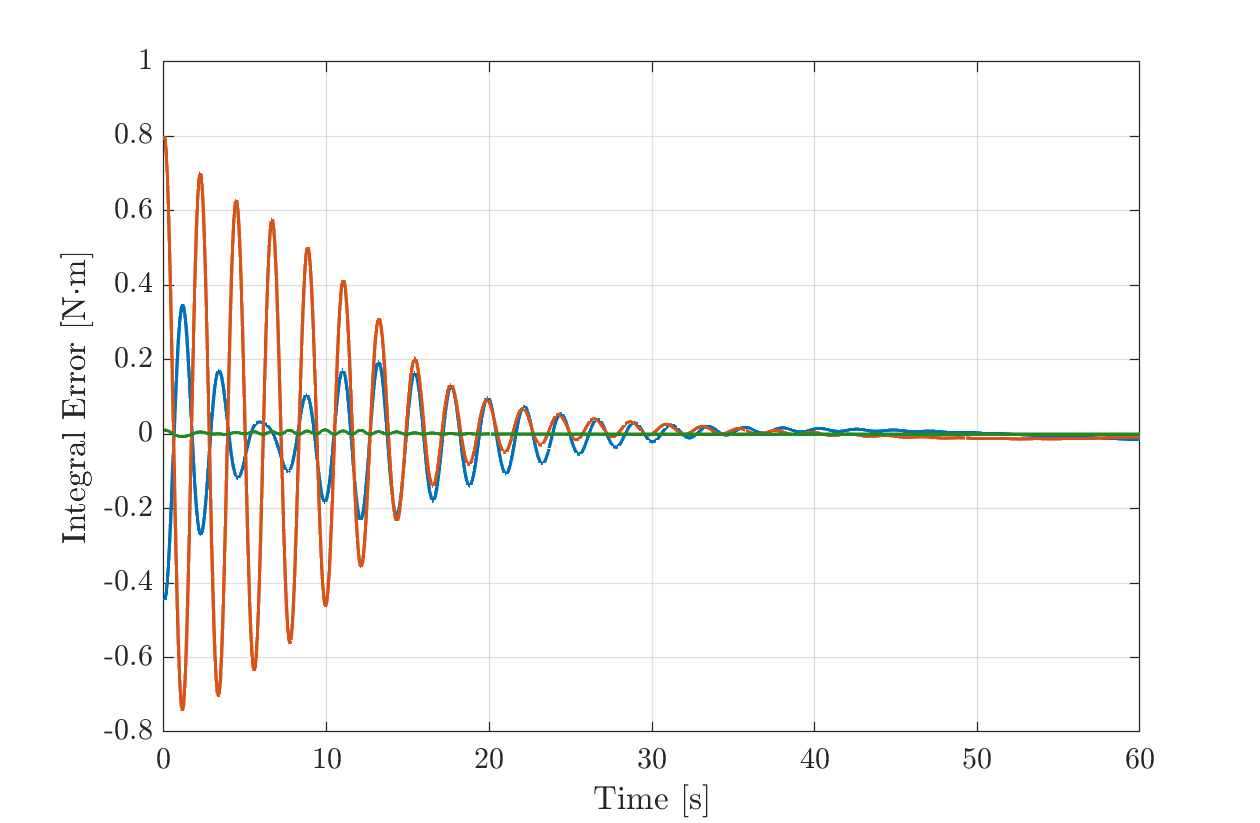
\includegraphics[width=0.9\linewidth]{plots/PID_sim_integral_error.png}
    \caption{Projected integral error during a simulated PID run}
    \label{fig:PID_sim_integral_error}
\end{figure}

\begin{figure}[h]
    \centering
    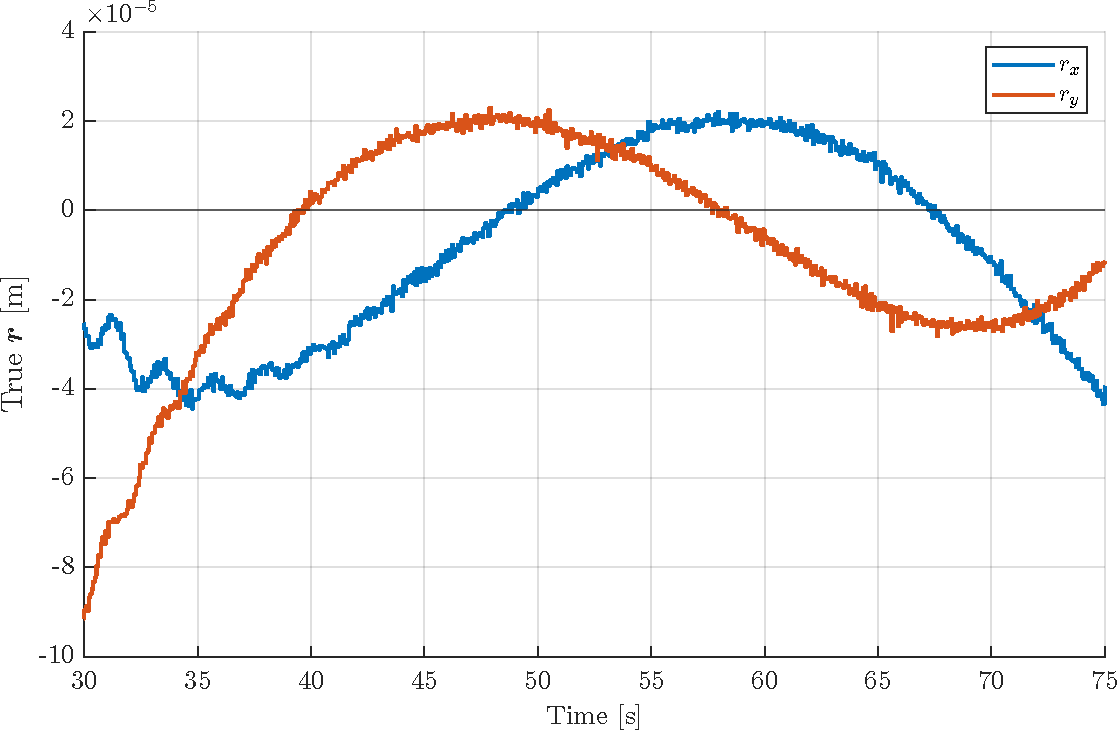
\includegraphics[width=0.9\linewidth]{plots/PID_sim_oscillations.pdf}
    \caption{Simulated PID scillatations about $\bm{r}=0$ at steady state}
    \label{fig:PID_sim_oscillations}
\end{figure}


From \Cref{fig:PID_sim_results} alone it can be inferred that the controller has horizontally balanced the platform. However, to further validate the performance of the balancing method, various values from the truth model are plotted. \Cref{fig:PID_sim_integral_error} shows the projected integral error of the controller. It is clear the integral action does indeed learn and compensate for the initial gravitional torque $\bm{\tau}_{g,0}$. The effects of the simulated controller can also be seen, with the 15 Hz discrete time integrator causing noise at steady state.


\Cref{fig:PID_sim_oscillations} shows the true value of $r_x$ and $r_y$ at steady state. The values begin to oscillate with a fairly constant amplitude about the desired values of $r_x = r_y = 0$. A variety of factors here prevent further convergence. The discretization of the controller, noise in the sensor readings, and lag in the control loop all limit the performance of the system. In a real hardware test, the operator will end the balancing procedure once the sliding mass positions have converged. Thus, the final value $r_x$ and $r_y$ will land at a random position along the two curves in \Cref{fig:PID_sim_oscillations}. The ampltiude of these oscillations places a bound on the final balancing results. In this case, $r_x$ and $r_y$ are bounded by $\pm4\times10^{-5}m$, so in the worst case, the simulated PID balancing procedure has still reduced the horizontal inbalance by two orders of magnitude.

Next the experimental PID results on the SADS are considered. \Cref{fig:PID_hardware_results} shows the same system states during the balancing procedure. The system qualitatively behaves in a similar manner to the simulated results. The platform's roll, pitch, and horizontal body rates converge towards zero and the sliding mass positions additionally converge towards a constant value. The values for all experimental system states are all generally smaller in magnitude compared to the simulated values from \Cref{fig:PID_sim_results}, indicating the initial imbalance was smaller.  

While a plot like \Cref{fig:PID_sim_oscillations} cannot be recreated in an experimental test, the oscillations of $\Delta\bm{d}$ in \Cref{fig:PID_hardware_results} can be converted into oscillations of $\Delta\bm{r}$ using \Cref{equation:delta_d_sol}. This leads to $\Delta\,r_x$ and $\Delta\,r_y$ being bounded by $\pm2.5\times10^{-5}m$, which is similar to simulated value of $\pm4\times10^{-5}m$. This suggests good alignment between the simulated system and the experimental system, however it is unknown if the oscillations in the experimental test are about the desired values of $r_x = r_y = 0$.




\section{Underactuated Adaptive Control}

Next, the adaptive control method is implemented into the same simulation. Attempts to simulate this method however quickly created numerical instability within the simulation. To alleviate this, all sources of error discussed in \Cref{sec:sim_setup} are temporarily removed from the simulation which results in \Cref{fig:adaptive_sim_success}. The results here indicate the implemented control law works under the mathmatically ideal case. $\bm{\omega}_p$ converges to $\bm{0}$ and the sliding mass converge to the position that minimizes $r_x$ and $r_y$. However, the sliding mass velocites and rapid oscillations of the platform are not physically feasible. This behaviour is identical to the results of \cite{silva_filtering_2018} and \cite{hudson_dynamic_2019}, which both attempt to simulate the same adaptive controller. After many attempts to diagose the source of instability, it remains unclear what differs between the original implementation of this balancing method in \cite{chesi_automatic_2014}, and the implementation in \cite{silva_filtering_2018}, \cite{hudson_dynamic_2019}, and this work.

\begin{figure}[p!]
    \centering
    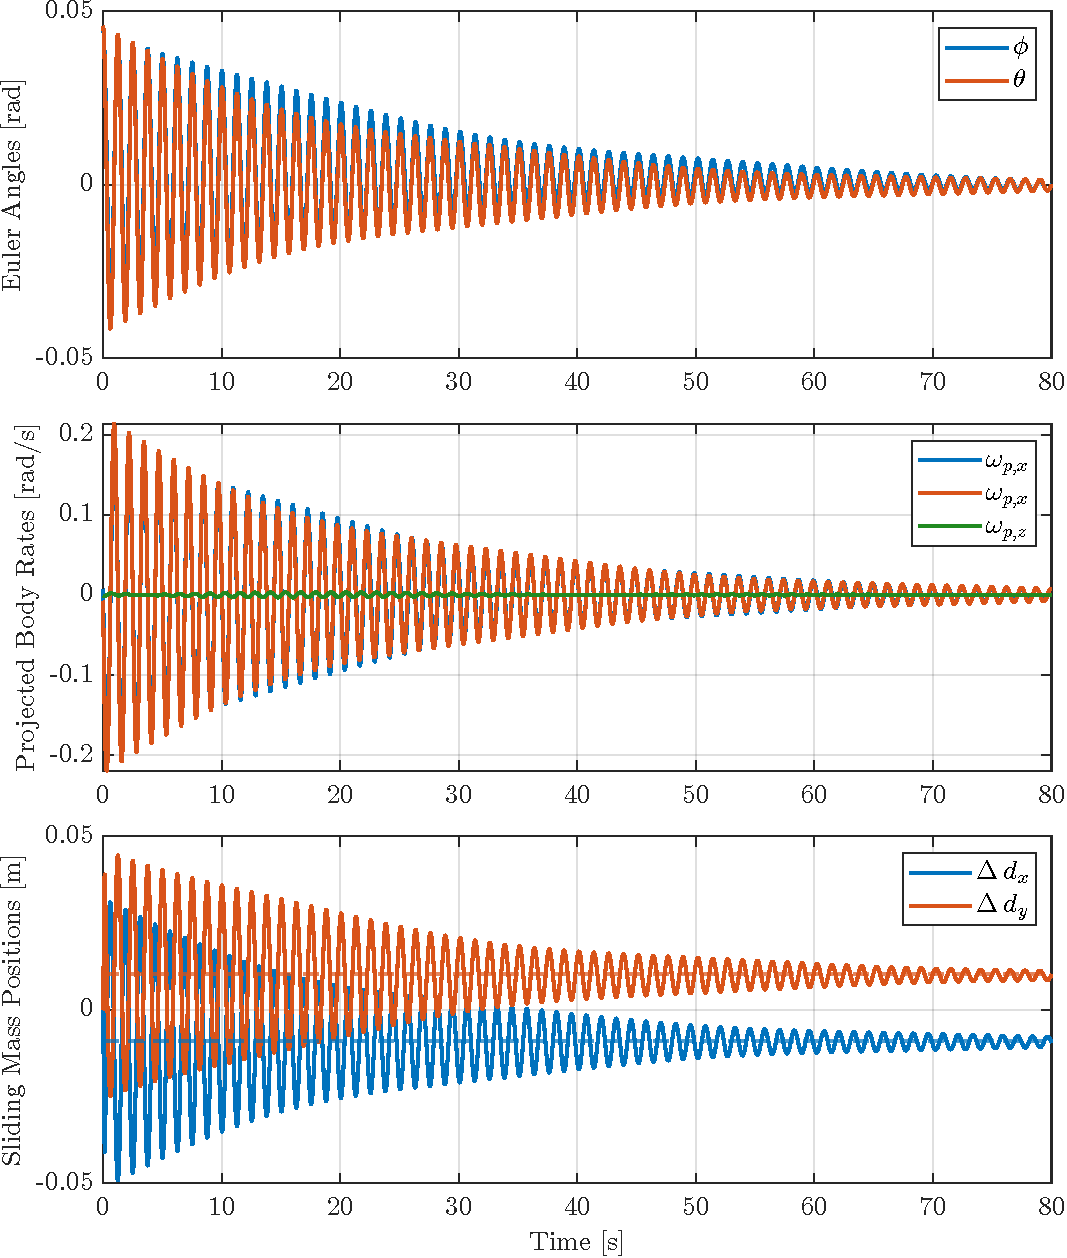
\includegraphics[width=\linewidth]{plots/adaptive_sim_success.pdf}
    \caption{Simulated underactuated adaptive control results using a simplified model}
    \label{fig:adaptive_sim_success}
\end{figure}

\begin{figure}[p!]
    \centering
    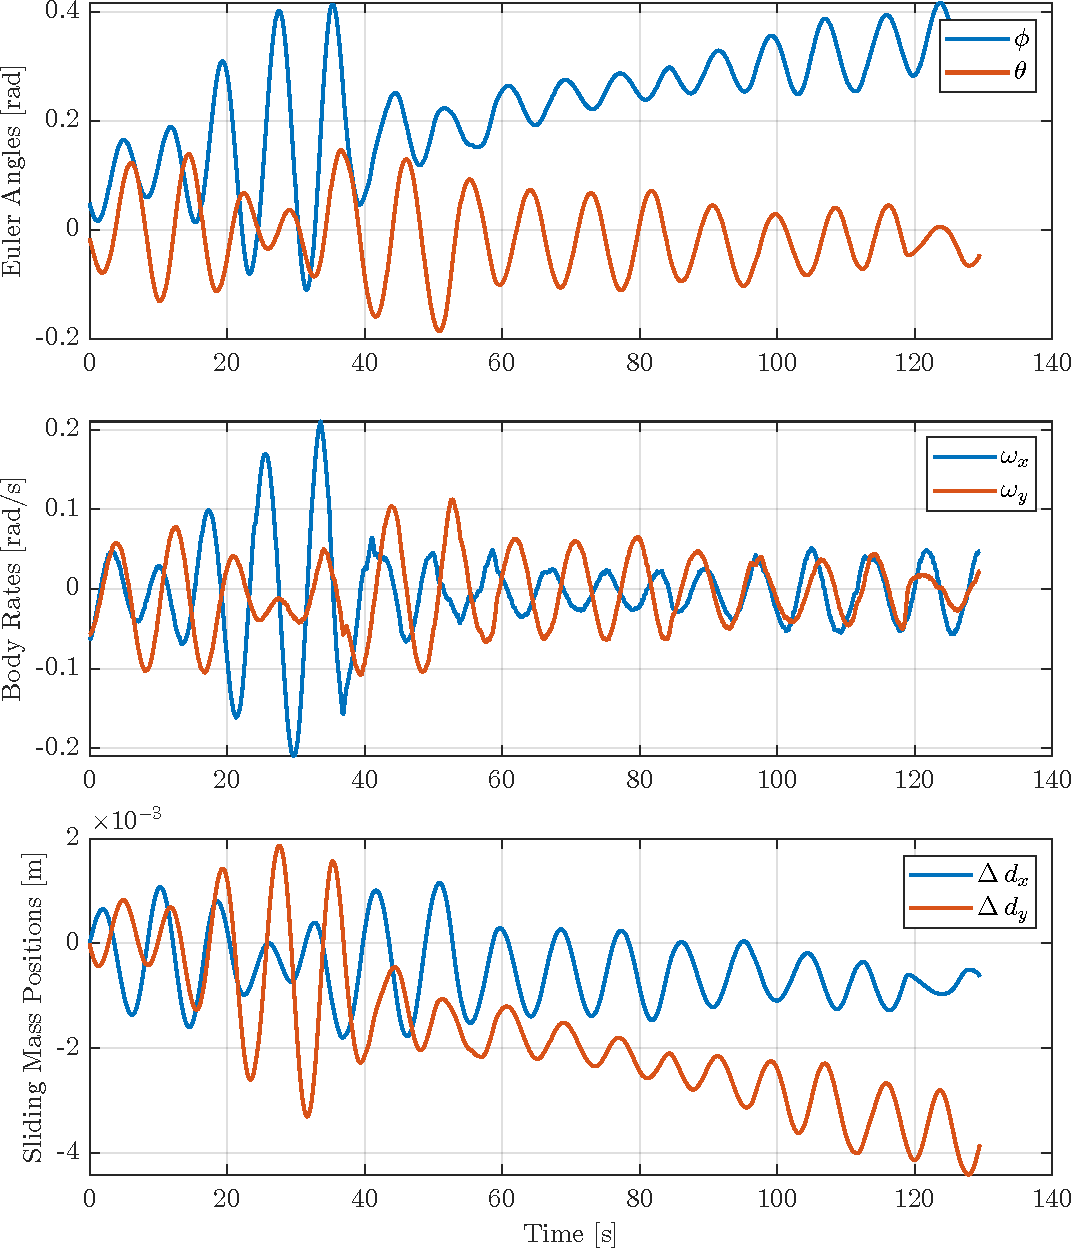
\includegraphics[width=\linewidth]{plots/adaptive_hardware_failure.pdf}
    \caption{Experimental results using underactuated adaptive control}
    \label{fig:adaptive_hardware_failure}
\end{figure}

\begin{figure}[h]
    \centering
    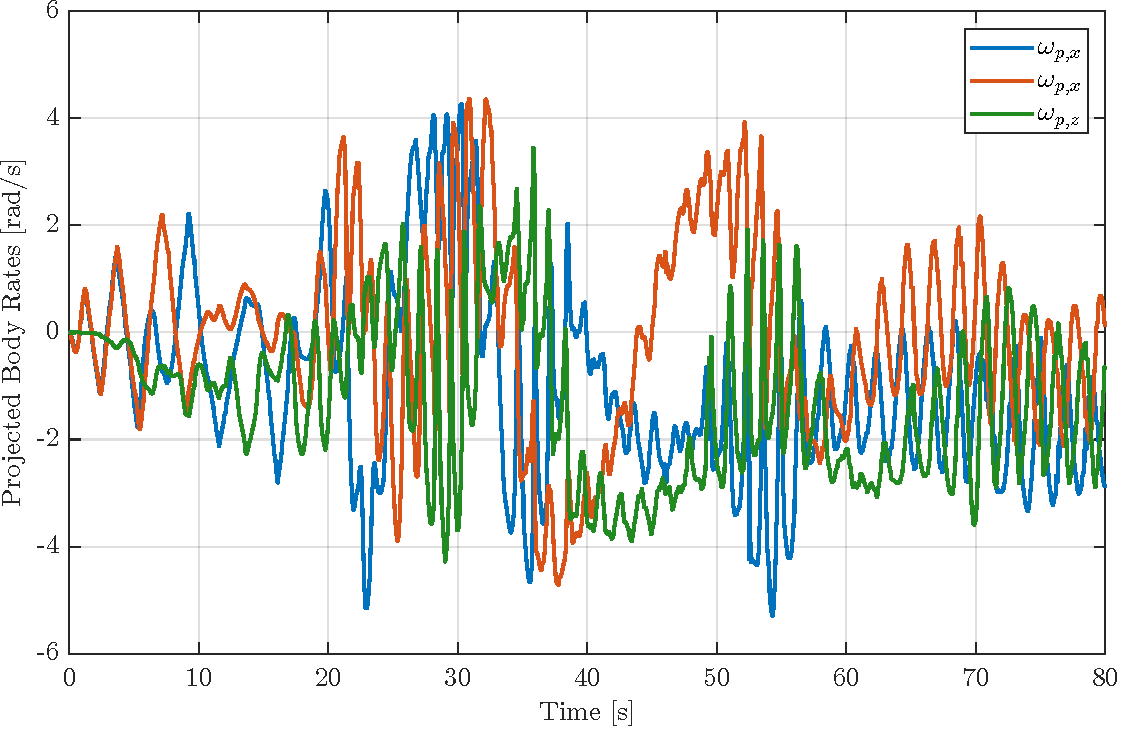
\includegraphics[width=0.9\linewidth]{plots/adaptive_sim_failure.pdf}
    \caption{Simulated underactuated adaptive control results with sensor dyanmics and onboard filtering modeled}
\end{figure}

Given the relative ease of changing control laws in the Matlab/Simulink environment, the underactuated adaptive control method is still implemented on the SADS to experiment which is seen in \Cref{fig:adaptive_hardware_failure}. Even with exensive tuning of the control gains, the simulator is generally unstable. The roll of the simulator at 120 seconds peaks at 0.4 radians, which is just beyond the $20^{\circ}$ safety limit of the test setup. In fact, \Cref{fig:adaptive_hardware_failure} shows the longest of the attempts that all were manually ended due to the simulator leaving its roll and pitch travel limits. Given the success of the PID method which has the identical goal of horizontally balancing the simulator, it was eventually decided to leave further investigation into the adaptive method as future work.  


\section{Vertical Inbalance Estimation with Kalman Filtering}


\begin{figure}[h]
  \centering
  \begin{subfigure}[t]{0.47\textwidth}
    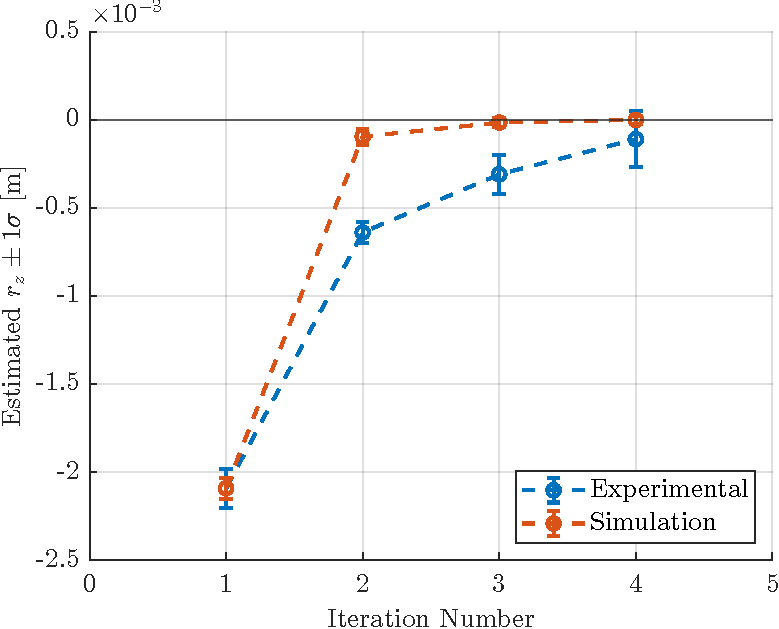
\includegraphics[width=\linewidth]{plots/UKF_comparison.pdf}
  \end{subfigure}\hfill
  \begin{subfigure}[t]{0.47\textwidth}
    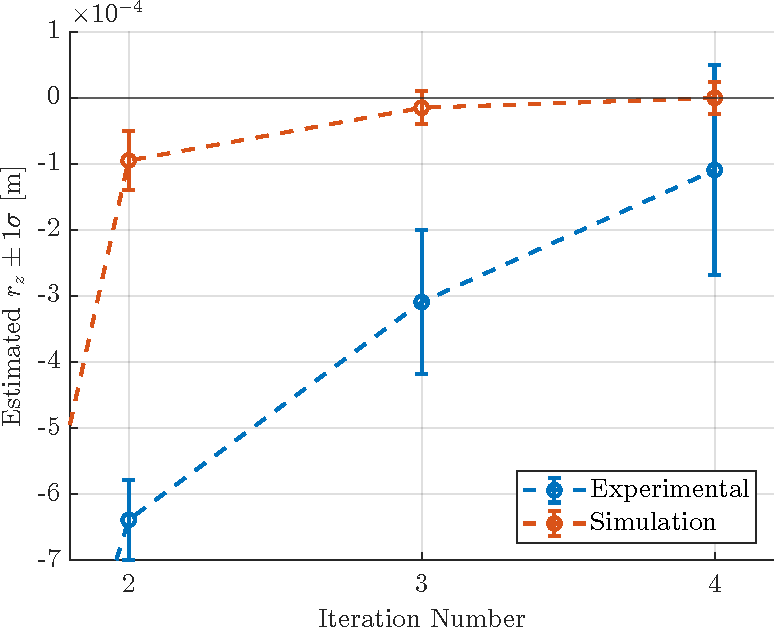
\includegraphics[width=\linewidth]{plots/UKF_comparison_zoomed.pdf}
  \end{subfigure}
  \caption{Filter results over multiple iterations, zoomed in on right}
  \label{fig:UKF_comparison}
\end{figure}


With the underactuated PID controller successfully horizontally balancing the platform, the UKF is then used to estimate the vertical inbalance. The free tumbling body rates of the platform are used as the filter input, with simulated tumbling data being used first to verify convergence. \Cref{fig:UKF_hardware_results} shows the filters output and $1\sigma$ confidence interval, where $\sigma$ is computed from the covariance matrix as $\sigma=\sqrt{P_k(7,7)}$. The filter shows strong convergence as $r_z$ is adjusted between each run in simulation. 

After filter convergence was demonstrated in simulation, real tumbling data from the SADS is used as input. The filter output over time during two selected iterations are shown in \Cref{fig:UKF_hardware_results}. \Cref{fig:UKF_hardware_results_a} shows the very first iteration after PID balancing. The filter quickly converges on an estimate for $r_z$, and the corresponding $1\sigma$ window is again plotted to demonstrate the filter's confidence. \Cref{fig:UKF_hardware_results_b} shows the filter output just two iterations later, where $r_z$ simply oscillates about 0. While the simulated and experimental results show similar behaviour, the simulated filter confidence is significantly higher, potentially indicating the modeling in \Cref{sec:sim_setup} did not introduce enough error into the simulation. 

\begin{figure}[h]
  \centering
  \begin{subfigure}[t]{0.47\textwidth}
    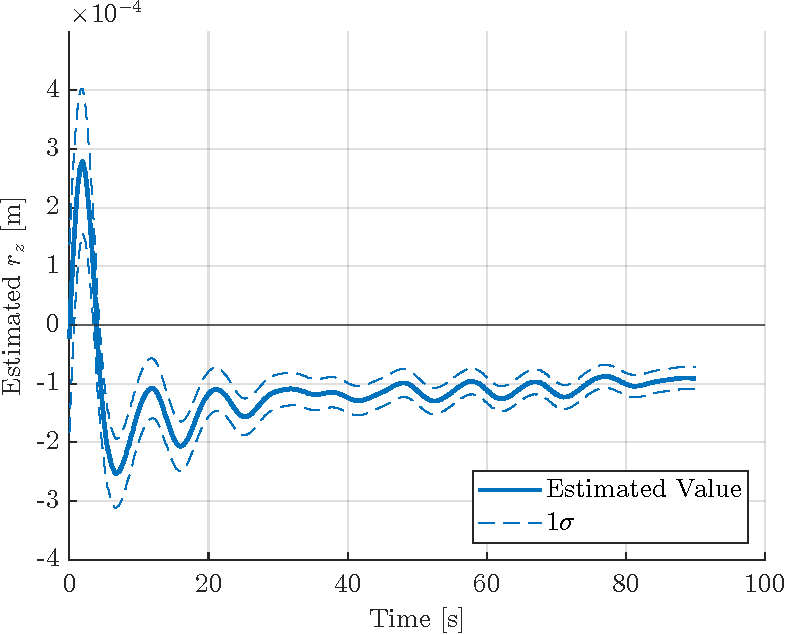
\includegraphics[width=\linewidth]{plots/UKF_hardware_success.pdf}
    \caption{Iteration successfully converging}\label{fig:UKF_hardware_results_a}
  \end{subfigure}\hfill
  \begin{subfigure}[t]{0.47\textwidth}
    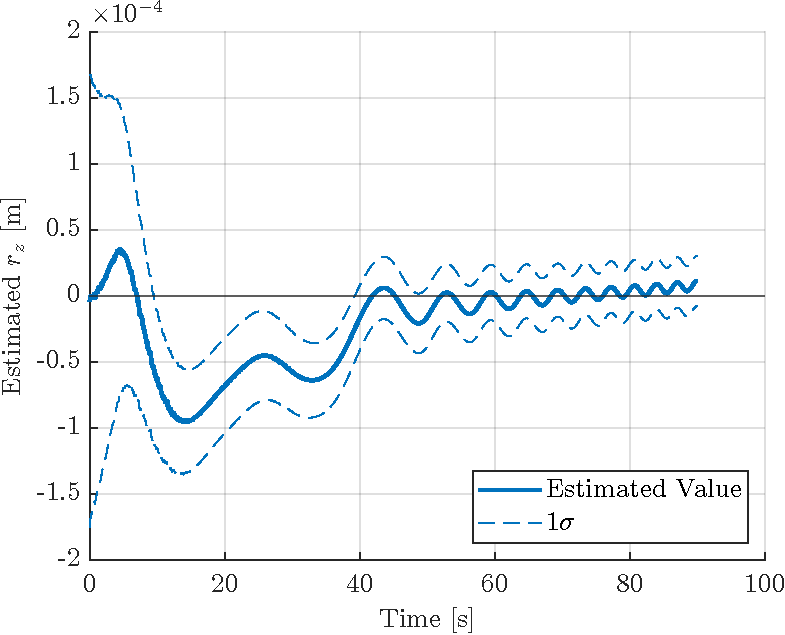
\includegraphics[width=\linewidth]{plots/UKF_hardware_failure.pdf}
    \caption{Iteration failing to converge}\label{fig:UKF_hardware_results_b}
  \end{subfigure}
  \caption{Experimental filter output during vertical inbalance estimation}
  \label{fig:UKF_hardware_results}
\end{figure}

In general as the true value of $r_z$ shrinks, the filter's ability to estimate $r_z$ also decreases. This is further demonstrated in \Cref{fig:UKF_comparison}, where the estimated values clearly tend towards 0, but the magnitude of the confidence interval starts to grow, even including positive values for $r_z$. This is important to consider when vertically balancing the simulator. During experimental tests it was observed the simulator could begin to tip over -- similar to an inverted pendulum -- when compensating for very small values of $r_z$. To avoid this behaviour, it became beneficial to only accept filter outputs where $\sigma$ is approximately less than $0.5r_z$. In practice, this means the vertical balancing procedure included two or three iterations before halting. 





\section{Passive Balancing Using Least-Squares Estimation}

The least-squares batch estimation method is first simulated using the intended four reaction wheel setup for the SADS. The platform's state during a batch collection run is shown in \Cref{fig:LSR_sim_excitation}. The torque profile is designed to have the platform oscillate as close as possible to it's $\pm20^{\circ}$ travel limits for roll and pitch, while simultaneously not saturating the reaction wheels. Both of these goals are met in the example run shown.

\begin{figure}[h]
  \centering
  \begin{subfigure}[t]{0.47\textwidth}
    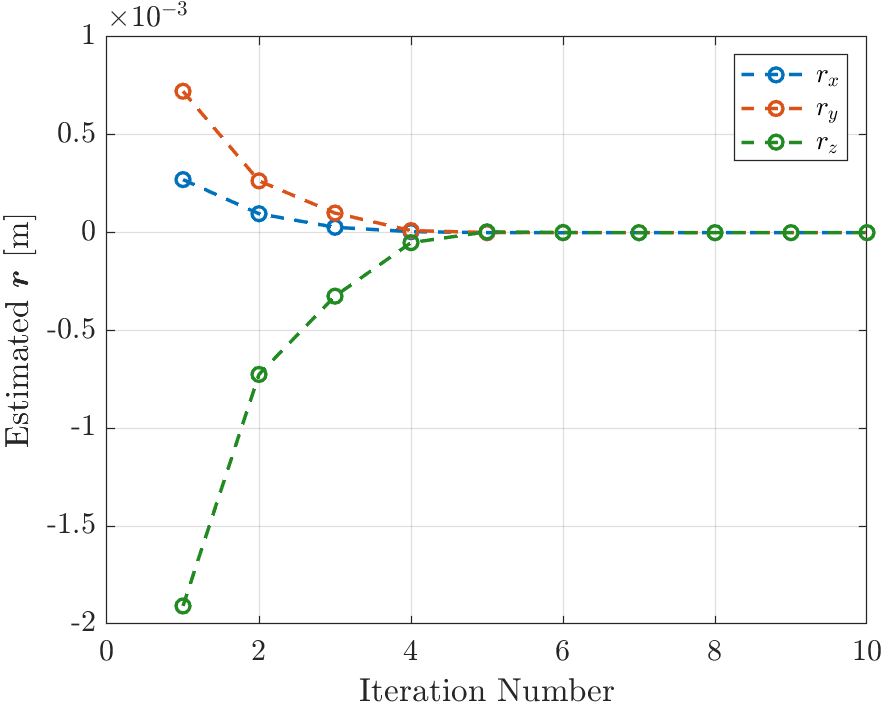
\includegraphics[width=\linewidth]{plots/LSR_sim_all_runs.png}
    \caption{All 10 iterations}\label{fig:LSR_sim_runs_a}
  \end{subfigure}\hfill
  \begin{subfigure}[t]{0.47\textwidth}
    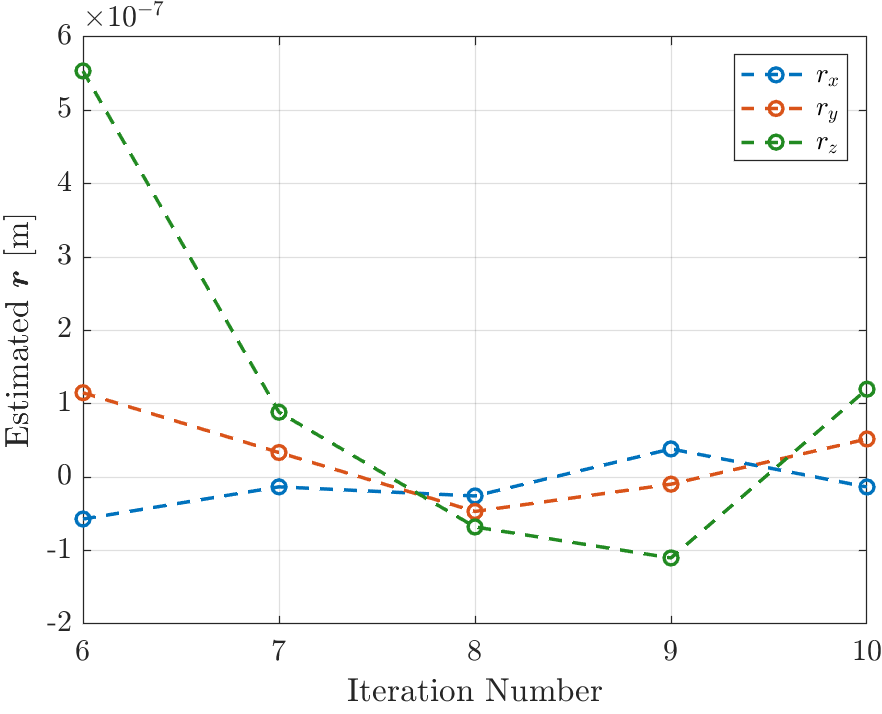
\includegraphics[width=\linewidth]{plots/LSR_sim_last_5_runs.png}
    \caption{Final 5 iterations}\label{fig:LSR_sim_runs_b}
  \end{subfigure}
  \caption{Simulated results of least-squares estimation method}
  \label{fig:LSR_sim_runs}
\end{figure}

\begin{figure}[p]
    \centering
    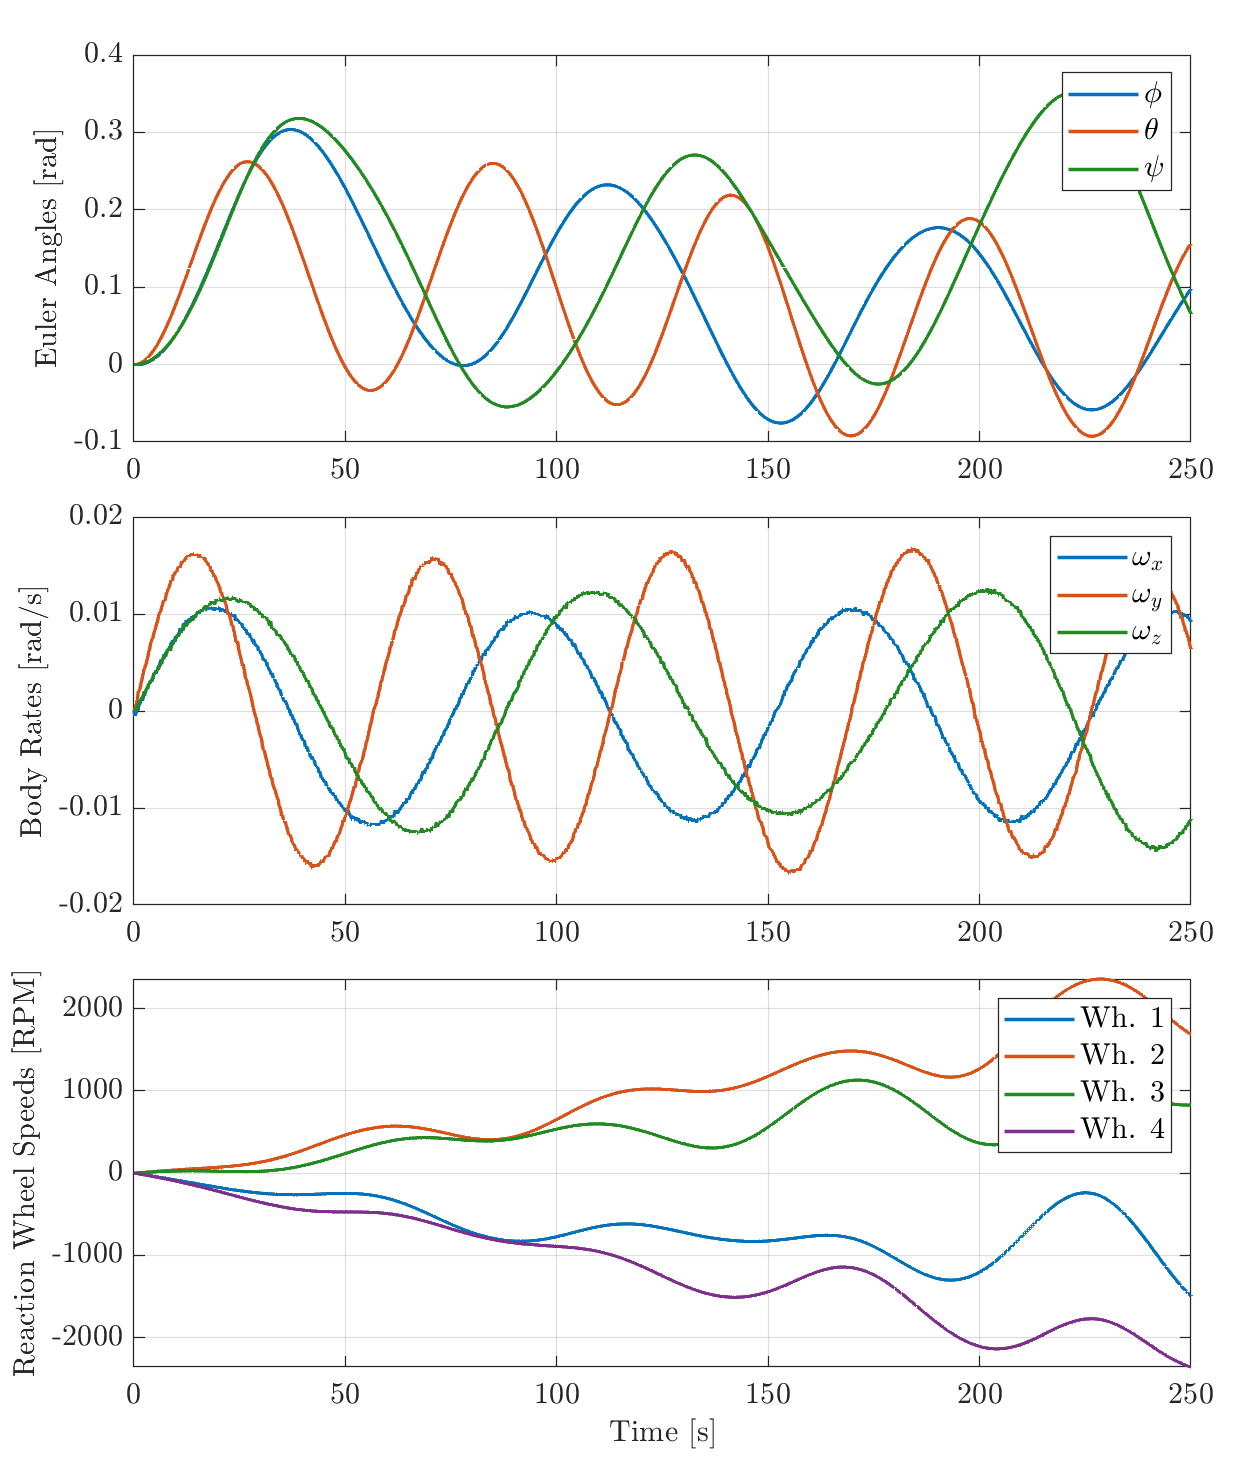
\includegraphics[width=\linewidth]{plots/LSR_sim_excitation}
    \caption{Simulated platform excitation during batch estimation}
    \label{fig:LSR_sim_excitation}
\end{figure}

\begin{figure}[p]
    \centering
    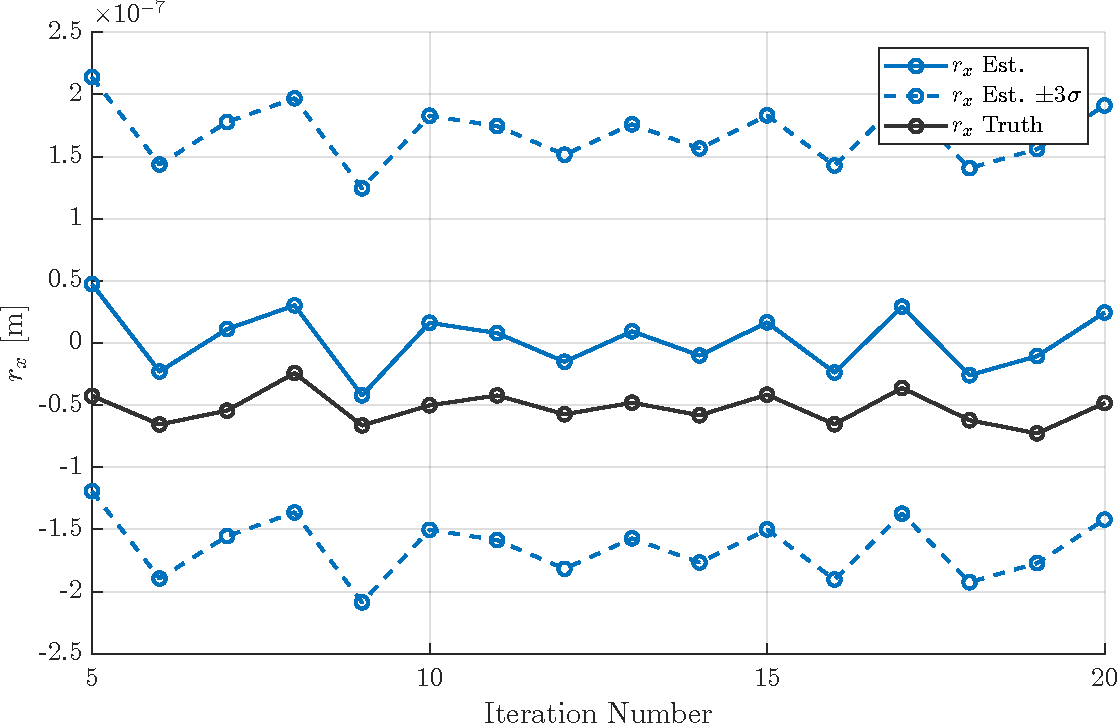
\includegraphics[width=\linewidth]{plots/LSR_sim_confidence.pdf}
    \caption{Simulated comparison between estimated and true values for $r_x$ using four reaction wheels}
    \label{fig:LSR_sim_confidence}
\end{figure}

\begin{figure}[p]
    \centering
    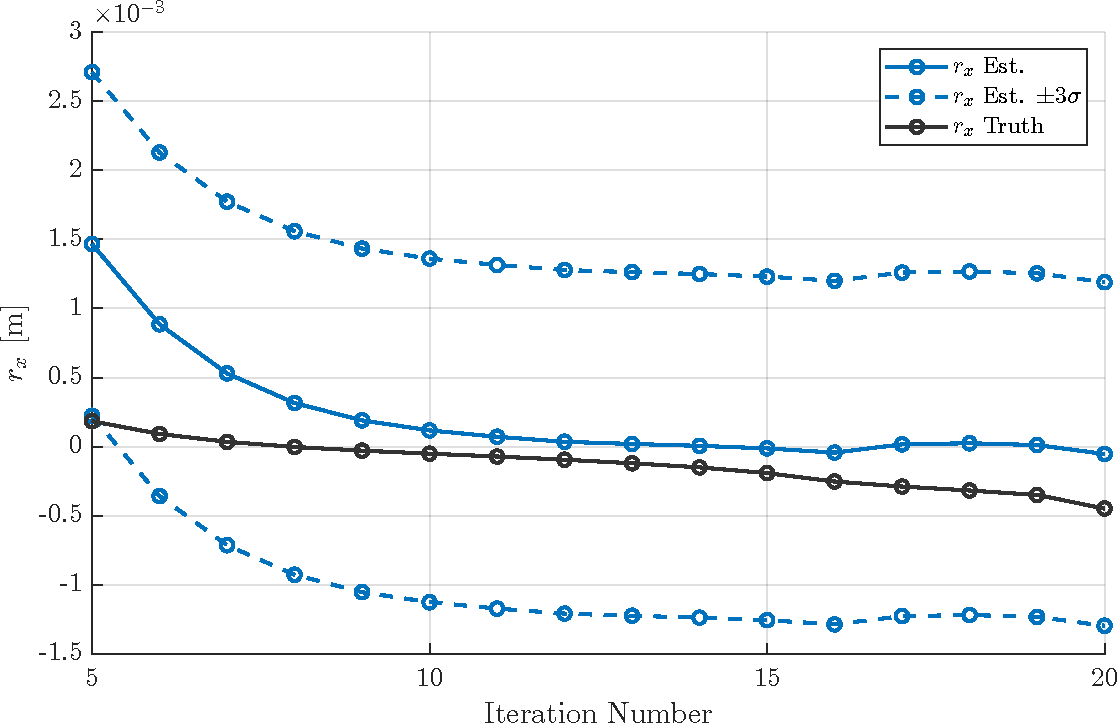
\includegraphics[width=\linewidth]{plots/LSR_sim_confidence_1_wheel.pdf}
    \caption{Simulated comparison between estimated and true values for $r_x$ using one reaction wheel}
    \label{fig:LSR_sim_confidence_1_wheel}
\end{figure}

\begin{figure}[p]
    \centering
    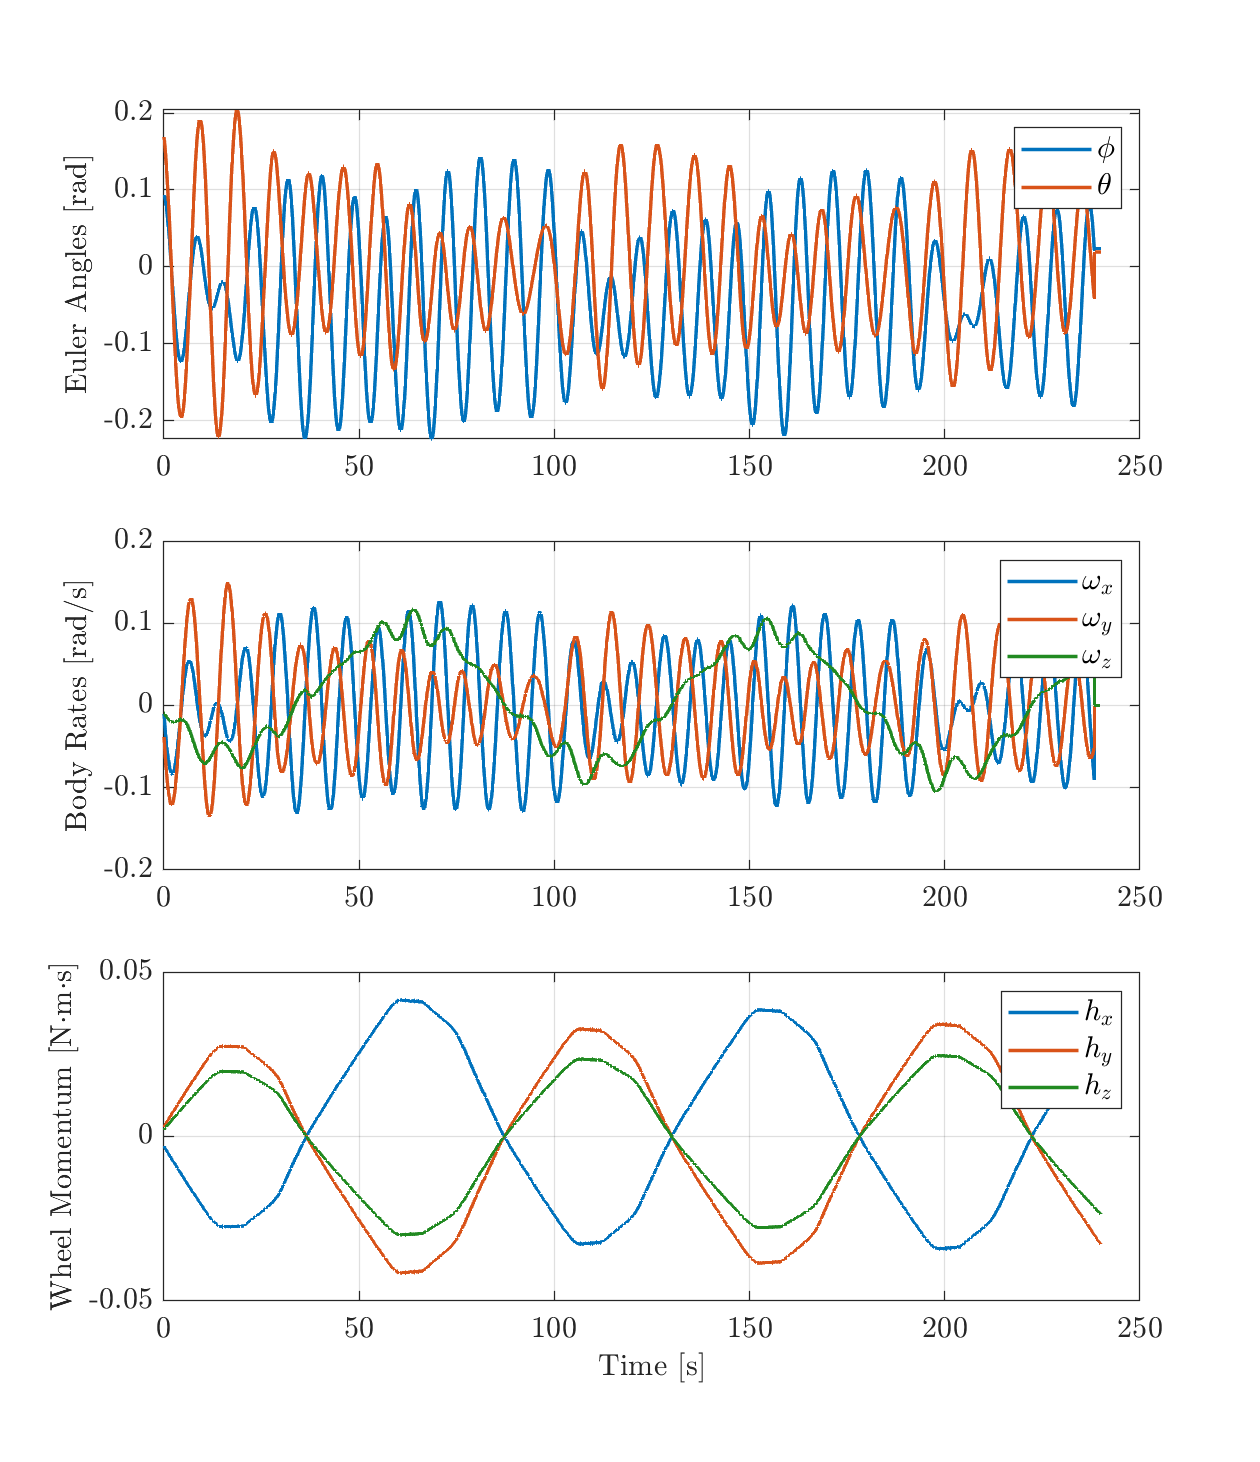
\includegraphics[width=\linewidth]{plots/LSR_hardware_excitation.png}
    \caption{Experimental platform excitation during batch estimation}
    \label{fig:LSR_hardware_excitation}
\end{figure}


The estimated value for $\bm{r}$ over the course 10 iterations is shown in \Cref{fig:LSR_sim_runs}. The estimated values rapidly converge during the first few iterations, and eventually begin to oscillatate about $\bm{r}=\bm{0}$. While the estimate of $\bm{r}$ converges towards $\bm{0}$ with some bound, this does not necessarily guarantee the true value of $\bm{r}$ is also converging towards. This is demonstrated in \Cref{fig:LSR_sim_confidence}, where the estimated value for $r_x$ is plotted directly against the true value of $r_x$ over many iterations. While the $r_x$ estimate oscillates about 0, the true value oscillates about a non-zero, constant value. This small error between the two is not measurable to the batch-estimation algorithm due to factors like sensor and process noise. 

The simulated procedure is repeated using one reaction wheel to better represent the limitations of the current experimental test setup. \Cref{fig:LSR_sim_confidence_1_wheel} shows the same comparison between the estimated value for $r_x$ and the true value over many iterations. Even with one wheel, the estimator qualitatively behaves the same. After about 12 iterations, the estimated value begins oscillating about $r_x=0$, while the true value oscillatates about a non-zero value. The key difference between the two is the scale of the estimated values and the associated error. The scaling of the y-axis in the one wheel test is four orders of magnitude larger than the four wheel test.

After convergence, the estimated values $r_x$, $r_y$, and $r_z$ are collected and the standard deviation $\sigma$ of the resulting sets are computed. The variance of the converged estimates provide a way to empirically measure the uncertainty of the estimator. Higher variance corresponds to a larger residual offset between the estimate and true center of mass. In both the four-wheel and one-wheel procedures, the true value of $r_x$ lies within the confidence interval created from $\sigma$, so the simulated results confirm that the batch estimator provides a consistent---but excitation-limited---way to approximate the true imbalance. 

\begin{table}[h!]
\caption{Performance summary of least-squares batch estimation}
\label{table:LSR_table}
\centering
\renewcommand{\arraystretch}{1.3} % row height
\begin{tabularx}{\textwidth}{
    >{\raggedright\arraybackslash}p{4.4cm}   % Test case
    >{\centering\arraybackslash}p{4.4cm}     % Sigma
    >{\centering\arraybackslash}X     % Mean error
}
\hline
\textbf{Test Case} &
\textbf{Std. Deviation, $\sigma$ [m]} &
\textbf{Mean Error [m]} \\
\hline
Simulated (4 Wheels) &
$2.99\times10^{-8}$ &
$4.55\times10^{-8}$ \\[1.2em]

Simulated (1 Wheel) &
$4.08\times10^{-6}$ &
$2.43\times10^{-4}$ \\[1.2em]

Experimental (1 Wheel) &
$1.60\times10^{-5}$ &
--- \\ 
\hline
\end{tabularx}
\end{table}

% sim four wheel sig: 2.99e-08
% sim four wheel mean err: 4.55e-08

% sim one wheel sig: 4.0834e-06
% sim one wheel mean err: 2.43e-04

% exp one wheel sig: 1.6e-05

\begin{figure}[h]
  \centering
  \begin{subfigure}[t]{0.47\textwidth}
    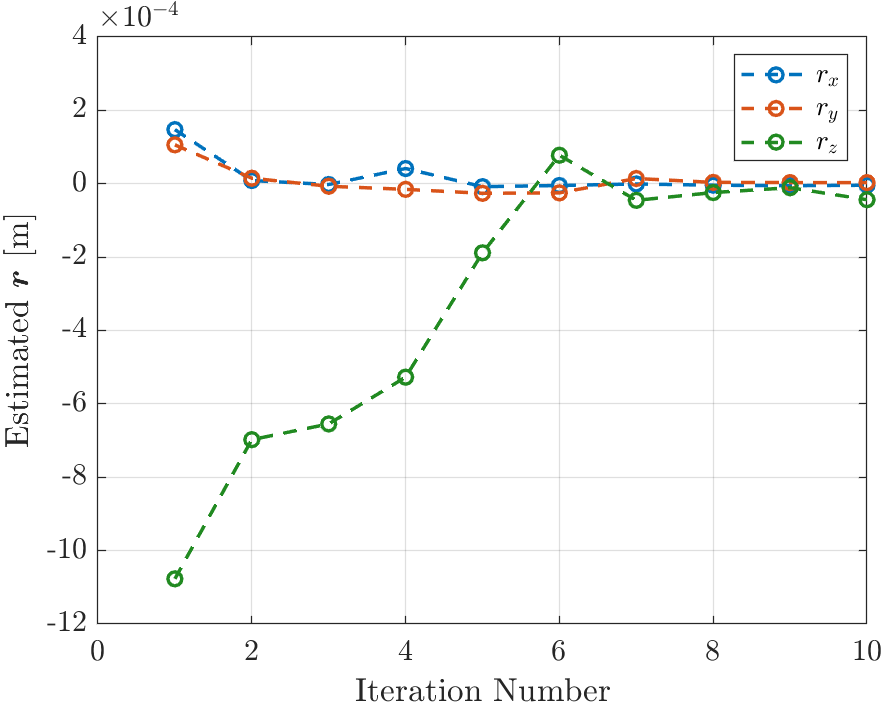
\includegraphics[width=\linewidth]{plots/LSR_hardware_all_runs.png}
    \caption{All 10 iterations}\label{fig:LSR_hardware_runs_a}
  \end{subfigure}\hfill
  \begin{subfigure}[t]{0.47\textwidth}
    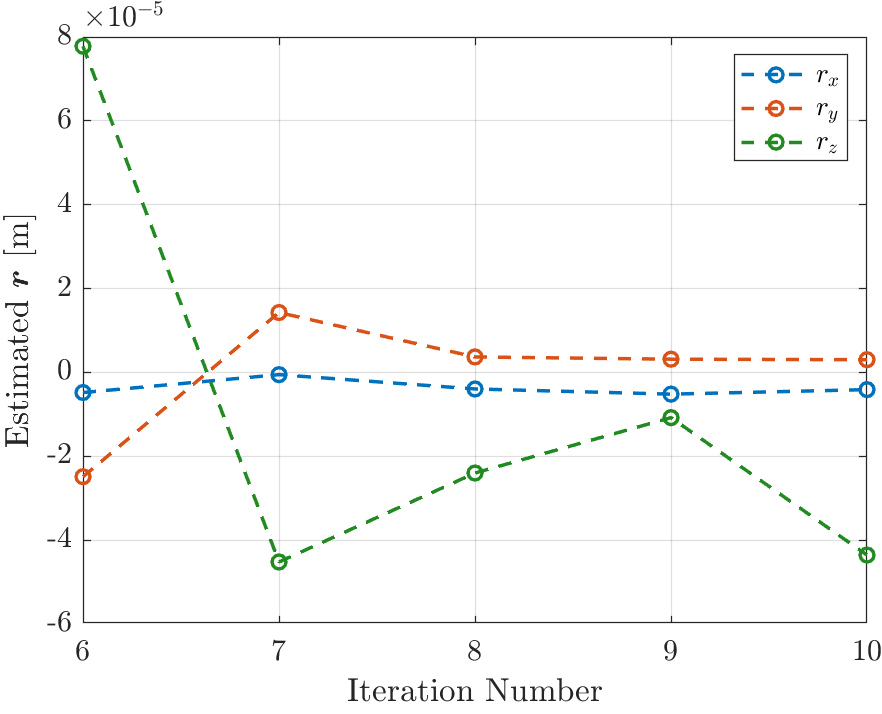
\includegraphics[width=\linewidth]{plots/LSR_hardware_last_5_runs.png}
    \caption{Final 5 iterations}\label{fig:LSR_hardware_runs_b}
  \end{subfigure}
  \caption{Experimental results of least-squares estimation method}
  \label{fig:LSR_hardware_runs}
\end{figure}

With the batch estimation algorithm verified using simulated values, the procedure is repeated on the SADS. The platform's state during a batch collection run is shown in \Cref{fig:LSR_hardware_excitation}. While the experimental setup includes only one reaction wheel, the SADS' pyramidal configuration means the one wheel contributes angular momentum to the system in all three axes of the body frame. 

The experimental results in \Cref{fig:LSR_hardware_runs} confirm that the least-squares batch estimator behaves consistently with simulation, converging toward a bounded region around the true center of mass. However, the significantly larger oscillations after convergence highlight the limitations of the current one-wheel setup. The results across the simulated and experimental tests are documented in \Cref{table:LSR_table}, where there is an increased variance in $\bm{r}$ compared the the simulated four-wheel results. While unmodeled system dynamics worsen the estimator, a majority of this difference can be attributed to the reduced excitation from using a single reaction wheel.

Despite these differences, the estimator demonstrates stable convergence and repeatable behavior, validating its practical feasibility for the SADS platform. These results establish a baseline performance level for the batch estimation method for which future iterations can be compared.

\section{Active Balancing Using Adaptive Control}

The last balancing method considered is the three-axis adaptive controller, which is applied in simulation only. The momentum trajectory of the simulator can be seen in \Cref{fig:three_axis_sim_excitation}. Each component of the desired angular momentum is chosen to be three sine waves with slightly varying amplitudes, phases, and frequencies. The resulting sliding mass positions are shown in \Cref{fig:three_axis_sim_positions}. The results here align well with work the completed in \cite{kim_automatic_2009}. $\Delta\,d_x$ and $\Delta\,d_y$ converge relatively quickly compared to $\Delta\bm\,d_z$, with convergence being on the order of hundreds of seconds. As also noted in \cite{kim_automatic_2009}, tuning the controller gains $\bm{K}$, and $\bm{\Gamma}$ proved to be somewhat difficult. Theoretically, increasing the adaptive gain $\bm{\Gamma}$ woud lead to faster convergence of $\Delta\bm{d}$, but higher gains led to instability in the platform. Choosing a desired momentum trajectory that leads to convergence of $\Delta\bm{d}$ while not quickly saturating the reaction wheels was also difficult balance to strike. Still, the desired values of the sliding mass positions are shown dashed in \Cref{fig:three_axis_sim_positions}, and the adaptive controller does indeed compensate for all three components of $\bm{r}$ simultaneously. The final emperically tuned gains used are 
$\bm{K} = \text{diag}(5,5,5)$ and  $\bm{\Gamma} = 10^{-5}\text{diag}(5, 5 , 80)$

\begin{figure}[p]
    \centering
    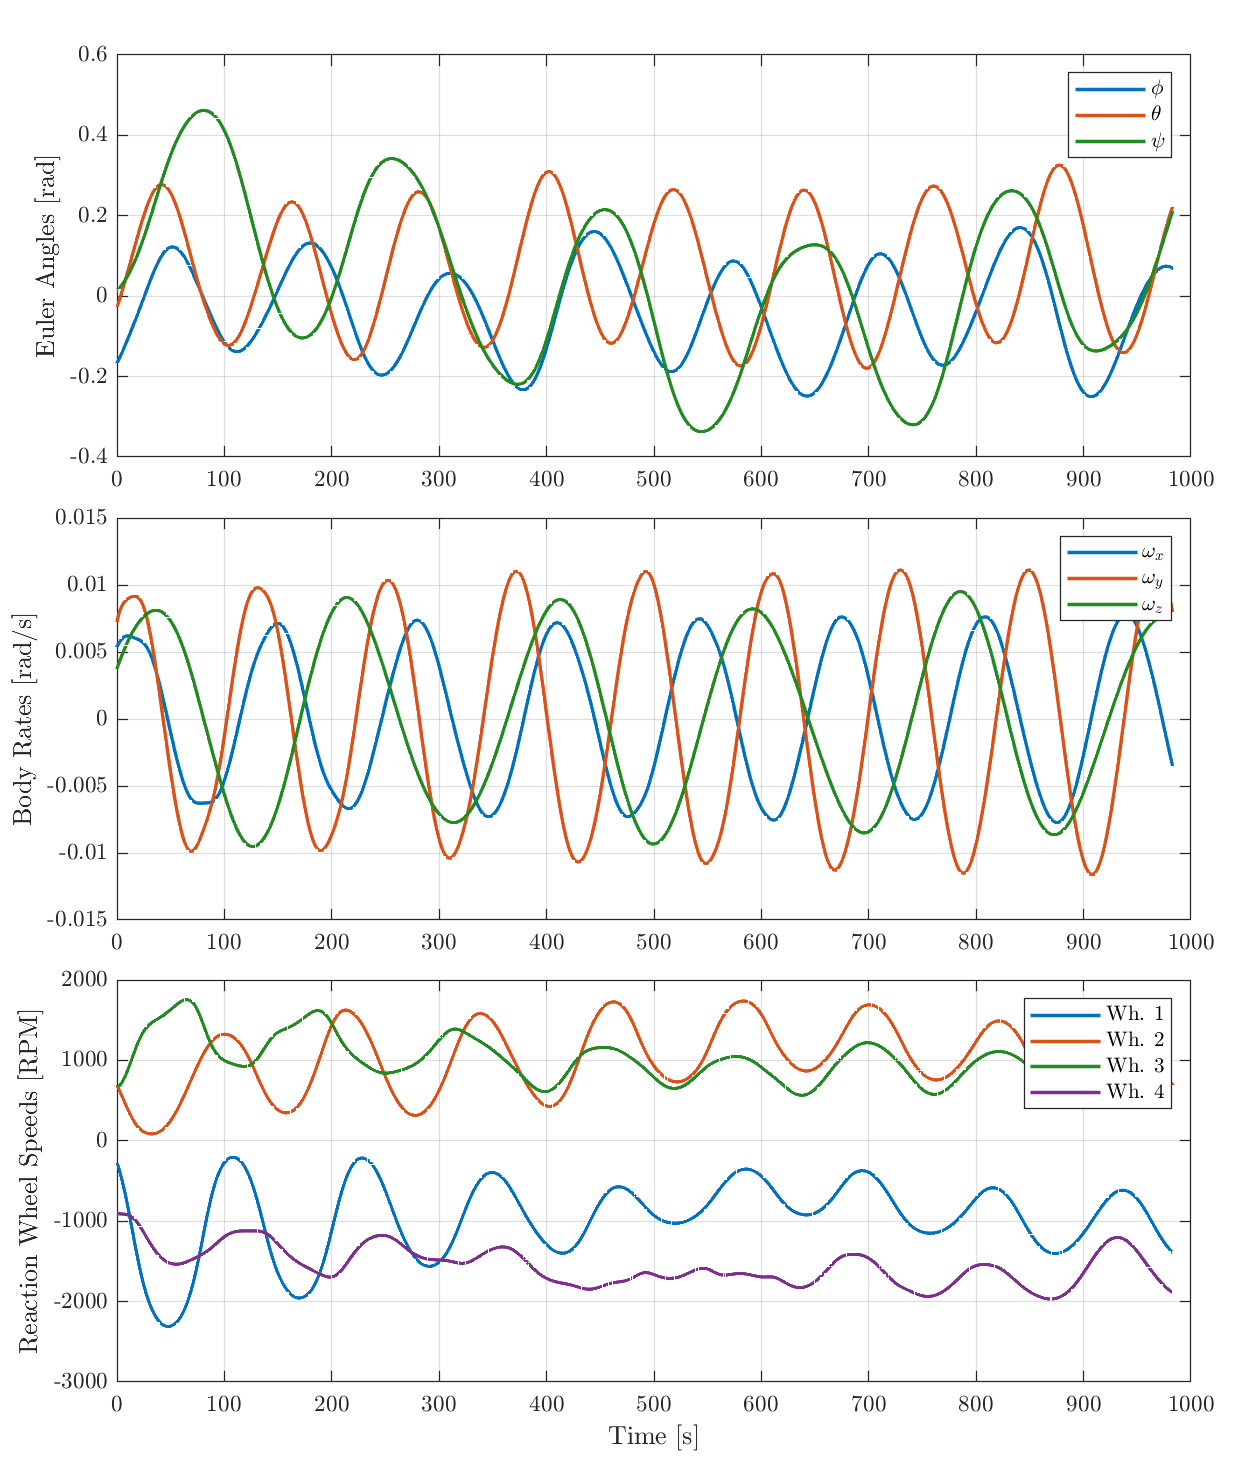
\includegraphics[width=\linewidth]{plots/three_axis_sim_excitation.png}
    \caption{Simulated platform excitation for 3-axis adaptive control}
    \label{fig:three_axis_sim_excitation}
\end{figure}

\begin{figure}[h]
  \centering
  \begin{subfigure}[t]{0.47\textwidth}
    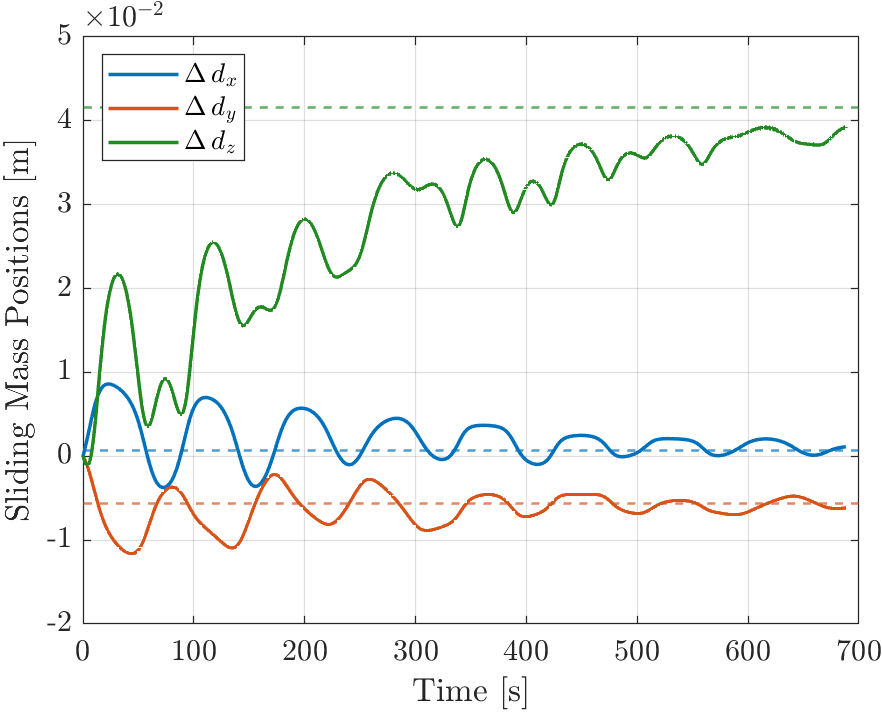
\includegraphics[width=\linewidth]{plots/three_axis_sim_positions_1.png}
    \caption{1st iteration}\label{fig:a}
  \end{subfigure}\hfill
  \begin{subfigure}[t]{0.47\textwidth}
    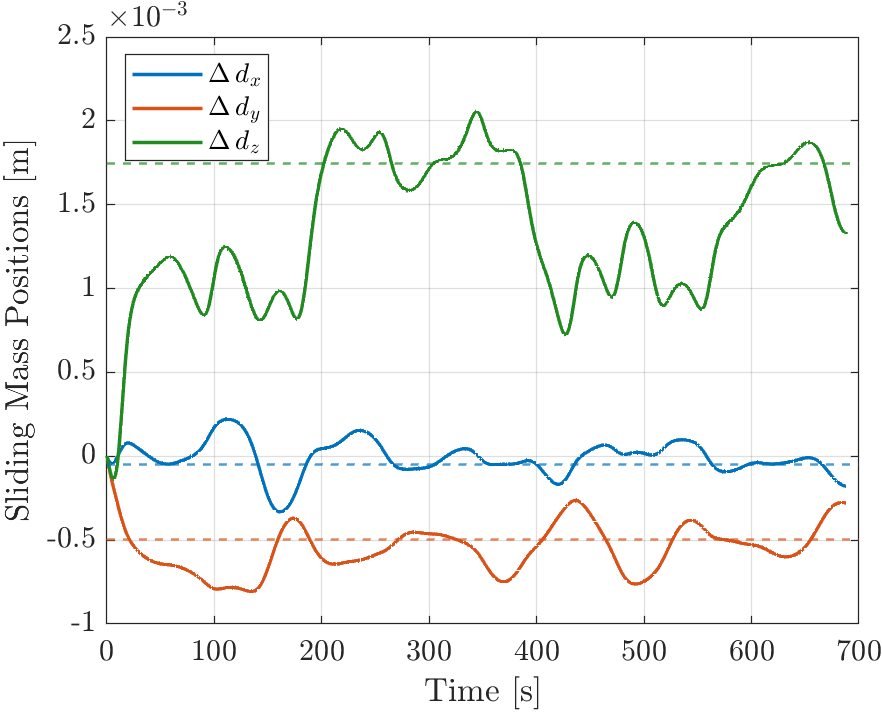
\includegraphics[width=\linewidth]{plots/three_axis_sim_positions_2.png}
    \caption{2nd iteration}\label{fig:b}
  \end{subfigure}
  \caption{Simulated sliding mass positions during 3-axis adaptive control}
  \label{fig:three_axis_sim_positions}
\end{figure}

\subsection{Verification}

Each balancing method described is verified using the external methods described in \Cref{sec:mbs_problem}. The simulator is first manually positioned such that $\phi=\theta=8^{\circ}$. It is then released to tumble freely, with the body rates being recorded. \Cref{fig:KE_post} shows the experimental computed kinetic energy of the simulator over about one minute of tumbling after both manual balancing and the hybrid PID method. The smaller oscillations in kinetic energy when using the hybrid PID method already indicates the magnitude of $\bm{r}$ has been succesfully decreased. \Cref{fig:torque_post} shows the gravity torque acting on the simulator during the same run. Again, the average torque magnitude using the hybrid PID method is significantly decreased compared to manually balancing the simulator. 

\begin{figure}[p]
    \centering
    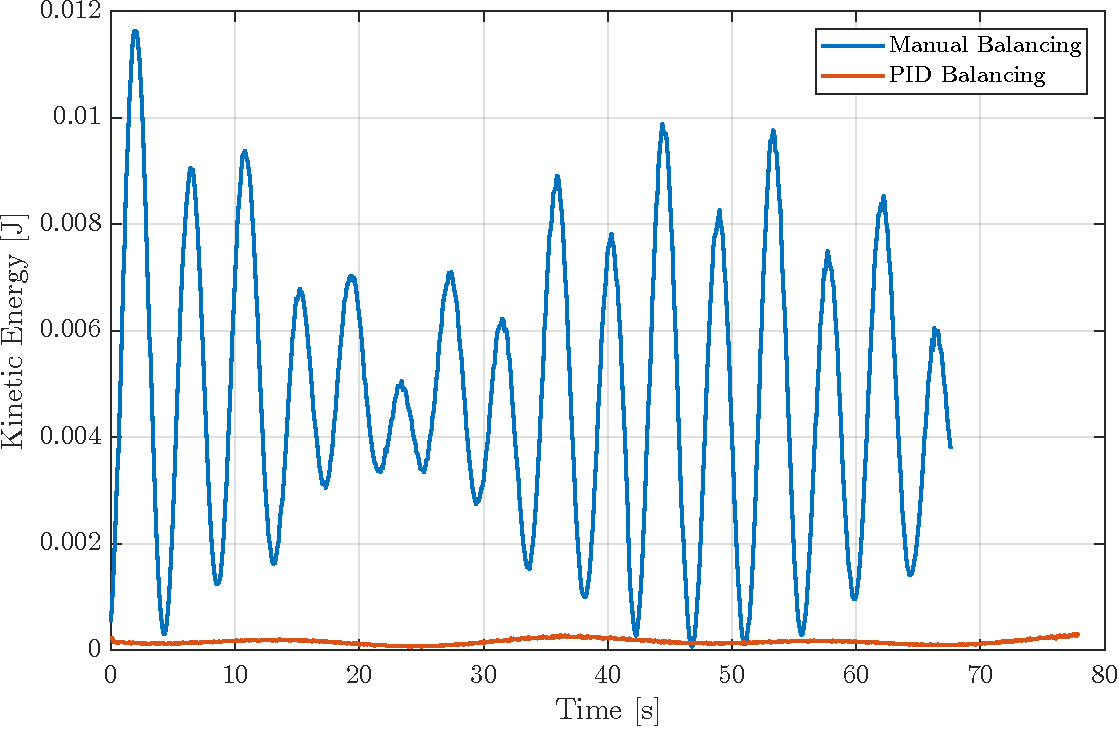
\includegraphics[width=0.85\linewidth]{plots/hardware_verification_KE.pdf}
    \caption{Kinetic energy of the simulator before and after using two-step PID balancing}
    \label{fig:KE_post}
\end{figure}

\begin{figure}[p]
    \centering
    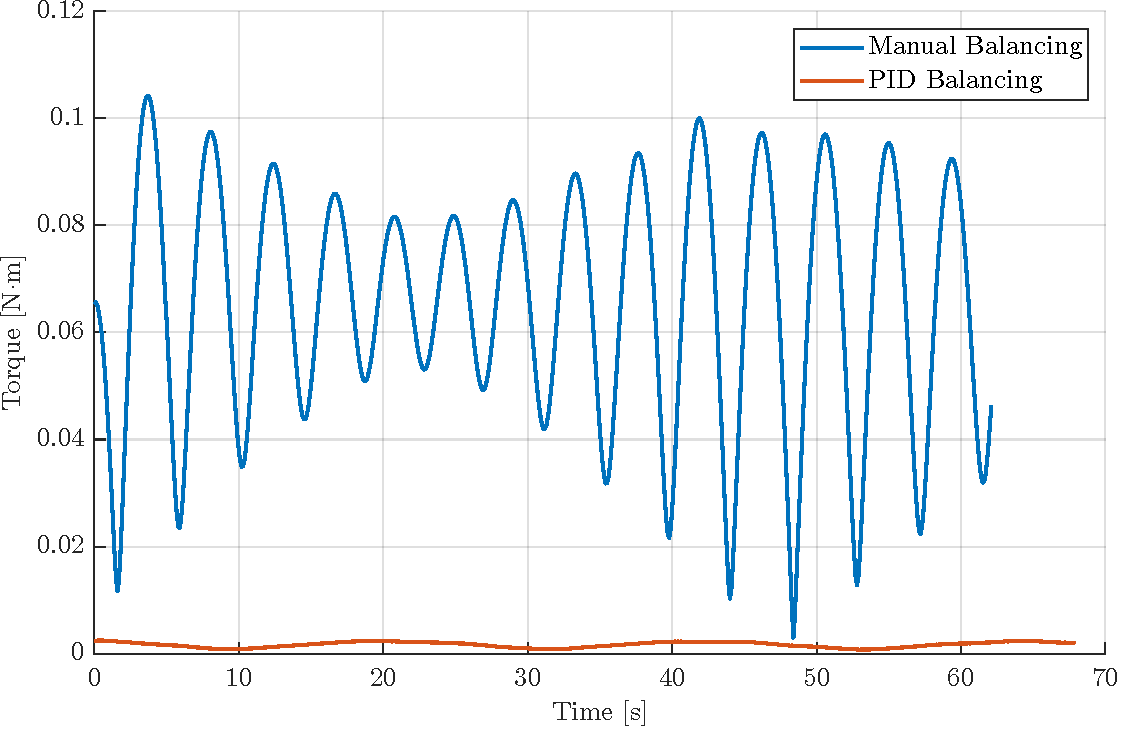
\includegraphics[width=0.85\linewidth]{plots/hardware_verification_torque.pdf}
    \caption{Norm of torque acting on the simulator before and after using two-step PID balancing}
    \label{fig:torque_post}
\end{figure}

This process is repeated at the end of each experimental balancing method. For simulated runs, the verification test is recreated by simply setting the initial conditions of the solver to use $\phi=\theta=8^{\circ}$. As discussed in \Cref{sec:PID_results}, there is a degree of randomness to the balancing results of any given procedure. For simulated results, this is addressed by using a Monte Carlo approach, where the inital conditions of the platform are varied slightly before the simulated balancing method is applied, leading to many resulting values of $\bm{r}$ after balancing. These $\bm{r}$ values are then used in the verification test and the results are averaged. For experimental tests, this is addressed by simply repeating the procedure and averaging the results. 

The final result for each method are documented in \Cref{table:final_results}. As expected, the manual balancing method shows the worst performance among all methods. The hybrid PID method shows the best performance among the experimental tests. It also shows similar results to the simulated version, further supporting agreement between the experimental and simulated systems. While the batch estimation with one wheel is superior to the manual balancing, it ultimately leads to poor balancing results compared the PID alternative, both in simulation and in the experimental tests. The best theoretical results are achieved by the batch estimation method with the full four wheel setup. It can be concluded that proper excitation of the platform is not just beneficial, but necessary, to achieve good results using batch estimation. 

The results achieved by Dam are generally worse than those found in this work. This is almost certainly a result of the hardware limitations of the SADS at the time, as discussed in \Cref{sec:SADS_history}. The reported $\pm3\sigma$ value for $r_z$ in Dam's work is $-1.581\pm0.0707mm$. This is about one order of magnitude worse than high-confidence UKF estimates for $r_z$ in this work (see \Cref{fig:UKF_hardware_results_a}). Without any way to finely control the positions of the sliding masses back in 2014, this was the best achievable result at the time. The improvements to the balancing hardware discussed in \Cref{chap:methodology} avoided theses issues all together. As a result, the best experimental results in this work (the hybrid PID method) are a direct improvement over the previous MBS design on the SADS.

\begin{table}[ht]
\caption{Comparison of Balancing Methods and Performance Metrics}\label{table:final_results}
\centering
\renewcommand{\arraystretch}{1.3}

\begin{tabularx}{\textwidth}{
    >{\raggedright\arraybackslash}p{4cm}
    >{\centering\arraybackslash}p{3cm}
    >{\centering\arraybackslash}X
}
\toprule
\textbf{Method} & \textbf{Avg. Torque [N·m]} & \textbf{max ($\Delta$KE) [J]} \\
\midrule
Manual Balancing & 0.0652 & 0.0116 \\ \addlinespace[0.2em]
Results from Dam & 0.0244 & 0.00782 \\ \addlinespace[0.2em]
PID + UKF Simulated & 0.00321 & 0.000965 \\ \addlinespace[0.2em]
PID + UKF Experimental & 0.00166 & 0.000236 \\ \addlinespace[0.2em]
Batch Estimation Simulated (4 wheels) & $3.89\times10^{-5}$ & 0.000116 \\ \addlinespace[0.2em]
Batch Estimation Simulated (1 wheel) & 0.0388 & 0.00296 \\ \addlinespace[0.2em]
Batch Estimation Experimental (1 wheel) & 0.0146 & 0.00226 \\ \addlinespace[0.2em]
3-Axis Adaptive Simulated & 0.00299 & 0.000741 \\ \addlinespace[0.2em]
\bottomrule
\end{tabularx}
\end{table}

\iffalse
SIM RESULTS ------------------------------
Results PID:
horizontal: 2.5e-5
verit 6.7e-7
KE = 0.00096508
torque = 0.0032123

Results Batch:
horizontal: 1e-7
vert: 2.2e-7
KE = 0.00011609;
torque = 3.8857e-05;

Results UKF
r_z = 6.784e-07

Results 3-axis
horizontal: 4.8261e-06
vertical: 9.7241e-05
KE = 0.00074126
torque = 0.0029949

HARDWARE RESULTS ----------------------------------
Results PID:
KE = 0.00023616
torque =  0.0016608;

Results Passive:
KE = 0.0022634
torque = 0.014569

Manual Balancing:
KE = 0.011555
torque = 0.065169

Dam:
KE = 0.0078203
torque = 0.0244

\fi